\chapter{Geraden und Ebenen}
\section{Wiederholung: Vektoren im Raum}

\subsection{Vektoren im Raum $\mathbb{R}^3$}

\begin{definition}
    Vektoren im Raum sind Zahlentripel, z. B. $$\vec{v} = \left(\begin{array}{c} x_1 \\ x_2 \\ x_3 \end{array}\right)$$ Wir geben Vektoren in Spaltenform an. Ein Vektor beschreibt eine Verschiebung im Raum. Ein Vektor lässt sich als Pfeil im Raum darstellen. Alle Pfeile, die zu einem Vektor gehören, sind zueinander parallel, gleichlang und gleich gerichtet.
\end{definition}

\noindent\rule{\textwidth}{1pt}

\textit{Beispiel:} Der Vektor $\vec{v} = \left(\begin{array}{c} 2 \\ -2 \\ 5 \end{array}\right)$ verschiebt einen Ausgangspunkt $A$ um 2 Einheiten in $x_1$-Achsenrichtung, um -2 Einheiten in $x_2$-Achsenrichtung und um 5 Einheiten in $x_3$-Achsenrichtung.

\subsection{Allgemeine Darstellung}

Allgemein wählen wir \textbf{\textendash{}} bezogen auf ein kartesisches Koordinatensystem \textbf{\textendash{}} einen beliebigen Anfangspunkt. Dann bewegen wir uns je nach Vorzeichen der Koordinaten \\[5pt]
um $\left|a_1\right|$ in Richtung (Gegenrichtung) der $x_1$-Achse, um $\left|a_2\right|$ in Richtung (Gegenrichtung) der $x_2$-Achse und um $\left|a_3\right|$ in Richtung (Gegenrichtung) der $x_3$-Achse und kommen zum Endpunkt es Pfeils.

\subsection{Berechnung eines Vektors: Anfangspunkt $A(a_1|a_2|a_3)$ und Endpunkt $B(b_1|b_2|b_3)$}

Wir berechnen: $\vv{v} = \vv{AB} = \left(\begin{array}{c} b_1 \\ b_2 \\ b_3 \end{array}\right) - \left(\begin{array}{c} a_1 \\ a_2 \\ a_3 \end{array}\right) = \left(\begin{array}{c} b_1 - a_1 \\ b_2 - a_2 \\ b_3 - a_3 \end{array}\right) = \left(\begin{array}{c} v_1 \\ v_2 \\ v_3 \end{array}\right)$

\begin{definition}
    Der \textbf{Ortsvektor} des Punktes $A$ geht vom Ursprung zum Punkt $A$ und hat die gleichen Koordinaten wie der Punkt $A$, d. h. $$\vv{OA} = \left(\begin{array}{c} a_1 \\ a_2 \\ a_3 \end{array}\right)$$
\end{definition}

\subsection{Verschiebung eines Dreiecks}

Gegeben sind die Punkte $A(1 \ |-1| \ 2), B(-2| \ 2 \ |-4), C(7 \ | \ 2 \ | \ 0) \text{ und } D(2 \ | \ 2 \ | \ 6)$.

Der Vektor $\vv{v} = \vv{AD} = \left(\begin{array}{c} 2 - 1 \\ 2 + 1 \\ 6 - 2 \end{array}\right) = \left(\begin{array}{c} 1 \\ 3 \\ 4 \end{array}\right)$ verschiebt das Dreieck $ABC$ auf das Dreieck $DEF$. Berechne die Koordinaten der fehlenden Punkte mit Hilfe der Vektorrechnung.

$\vv{OE} = \vv{OB} + \vv{AD} = \left(\begin{array}{c} -2 \\ 2 \\ -4 \end{array}\right) + \left(\begin{array}{c} 1 \\ 3 \\ 4 \end{array}\right) = \left(\begin{array}{c} -1 \\ 5 \\ 0 \end{array}\right) \Rightarrow E(-1| \ 5\ | \ 0)$ \qquad ($F$ analog zu $E$)

\subsection{Gegenvektor}

\begin{minipage}{0.65\textwidth}
    \begin{definition}
    Der \textbf{Gegenvektor} von \textbf{$\vv{a} = \vv{AB}$} ist \textbf{$-\vv{a} = -\vv{AB} = \vv{BA}$}.
    \end{definition}

    \textit{Beispiel:} $A(1 \ | -1 | \ 2), B(-2| \ 2 \ | -4)$ \\[3pt]

    $\vv{a} = \vv{AB} = \left(\begin{array}{c} -2 - 1 \\ 2 + 1 \\ -4 - 2 \end{array}\right) = \left(\begin{array}{c} -3 \\ 3 \\ -6 \end{array}\right); -\vv{a} = \left(\begin{array}{c} 3 \\ -3 \\ 6 \end{array}\right)$
\end{minipage}
\begin{minipage}{0.1\textwidth}
  \  
\end{minipage}
\begin{minipage}{0.25\textwidth}
    \begin{tikzpicture}
      \def\ul{0.52}
      \def\R{4}
      \def\ang{45}
      \draw[vector,black]
        (0,0) (0,0) node[below] {$A$} -- (\ang:\R) node[above] {$B$};
      \draw[vector,black,shift={(\ang-90:1)}]
        (\ang:\R) node[above] {$B$} -- (0,0) node[below] {$A$};
      \draw (0.75,1.5) node[above] {$\vv{a} = \vv{AB}$};
      \draw (3.2,0.25) node[above] {$-\vv{a} = \vv{BA}$};
    \end{tikzpicture}
\end{minipage}

\begin{definition}[Nullvektor]
    Mit $\vv{0}$ bezeichnen wir den Nullvektor, d. h. den Vektor mit der Länge 0: $\vv{a} + (-\vv{a}) = \vv{0}$. 
\end{definition}

\subsection{Die Addition von Vektoren}

\begin{definition}
    Die Summe zweier Vektoren $\vv{a}$ und $\vv{b}$ ist wiederum ein Vektor und entspricht der Hintereinanderausführung (Verkettung) zweier Verschiebungen.
\end{definition}

\begin{minipage}{0.5\textwidth}
    Wir erhalten den \textbf{Summenvektor $\vv{a} + \vv{b}$}, indem wir den Anfang des Vektors $\vv{b}$ an die Spitze des Vektors $\vv{a}$ verschieben. Der Pfeil des Summenvektors $\vv{c} = \vv{a} + \vv{b}$ beginnt im Fußpunkt des Pfeils von $\vv{a}$ und endet an der Spitze des Pfeils von $\vv{b}$.
\end{minipage}
\begin{minipage}{0.05\textwidth}
    \
\end{minipage}
\begin{minipage}{0.4\textwidth}
    \begin{tikzpicture}[scale=0.85]
        \draw[vector, black] (0,0) -- (1,-1);
        \draw (0.5,-0.5) node[above] {$\vv{a}$};
    
        \draw[vector, black] (0,-3) -- (1.5,-1.5);
        \draw (0.65, -2.5) node[right] {$\vv{b}$};
    
        \draw[vector, black] (2,-2) -- (3,-3) node[text width=3.5cm, align=center, below] {Fuß von $\vv{b}$ an der Spitze von $\vv{a}$};
        \draw (2.5,-2.5) node[above] {$\vv{a}$};
        \draw[vector, black] (3,-3) -- (4.5,-1.5);
        \draw (3.75, -2.25) node[above] {$\vv{b}$};
    
        \draw[vector, black] (6,-2) -- (7,-3);
        \draw (7.2, -3.3) node[text width=3.5cm, align=center, below] {$\vv{a} + \vv{b} = \vv{c}$};
        \draw (6.5,-2.6) node[left] {$\vv{a}$};
        \draw[vector, black] (7,-3) -- (8.5,-1.5);
        \draw (7.6, -2.5) node[right] {$\vv{b}$};
        \draw[vector, black] (6,-2) -- (8.5,-1.5);
        \draw (7.1, -1.75) node[above] {$\vv{c}$};
        
    \end{tikzpicture}
\end{minipage}

Zeichnerisch gewinnen wir die Summe als Diagonalvektor des von $\vv{a}$ und $\vv{b}$ aufgespannten Parallelogramms.
    
Vektoren werden addiert, indem wir die einander entsprechenden Koordinaten addieren.

\subsection{Die Subtraktion von Vektoren}

\begin{minipage}{0.7\textwidth}
    Werden die Vektoren $\vv{a}$ und $\vv{b}$ durch zwei Pfeile mit \textbf{gleichem} Anfangspunkt dargestellt, dann entspricht $\vv{b} - \vv{a}$ dem Pfeil, der vom Endpunkt von $\vv{a}$ zum Endpunkt von $\vv{b}$ führt. Die Subtraktion eines Vektors entspricht der Addition des Gegenvektors.
\end{minipage}
\begin{minipage}{0.05\textwidth}
    \ 
\end{minipage}
\begin{minipage}{0.25\textwidth}
    \begin{tikzpicture}
        \draw[vector, black] (0,-2) -- (3,-1.75);
        \draw (1.5, -1.875) node[below] {$\vv{a}$};
        \draw[vector, black] (0,-2) -- (0.75,0);
        \draw (0.375, -1) node[left] {$\vv{b}$};
        \draw[vector, black] (3,-1.75) -- (0.75,0);
        \draw (1.6, -0.5) node[right] {$\vv{b} - \vv{a}$};
        
    \end{tikzpicture}
\end{minipage}

\subsection{Gesetze der Vektoraddition}

\begin{satz}[Kommutativgesetz]
    Bei der Vektoraddition dürfen wir die Summanden vertauschen, ohne dass sich das Ergebnis, die Vektorsumme ändert: $$\vv{a} + \vv{b} = \vv{b} + \vv{a}$$
\end{satz}
\begin{satz}[Assoziativgesetz]
    Bei Vektorsummen dürfen wir Klammern umsetzen oder weglassen, ohne dass sich am Ergebnis etwas ändert: $$(\vv{a} + \vv{b}) + \vv{c} = \vv{a} + (\vv{b} + \vv{c}) = \vv{a} + \vv{b} + \vv{c}$$
\end{satz}

\subsection{Geometrische Darstellung der Multiplikation eines Vektors mit einer reellen Zahl (Skalarmultiplikation)}

\begin{minipage}{0.7\textwidth}
    Sei $\vv{a} \in \mathbb{R}^3$ und $r \in \mathbb{R}$. Werden die Vektoren $\vv{a}$ und $r\cdot \vv{a}$  durch Pfeile im Raum dargestellt, dann gilt: Der zu $r\cdot \vv{a}$ gehörige Pfeil hat die $|r|$-fache Länge des zu $\vv{a}$ gehörigen Pfeils. $r$ heißt Skalar.

    Ist $\vv{a} \neq \vv{0}$, dann sind die beiden Pfeile gleichsinnig parallel, falls $r>0$, und ungleichsinnig parallel, falls $r<0$.
\end{minipage}
\begin{minipage}{0.05\textwidth}
    \ 
\end{minipage}
\begin{minipage}{0.25\textwidth}
    \begin{tikzpicture}
        \draw[vector, black] (0,-2) -- (1,-1);
        \draw (0.55,-1.3) node[left] {$\vv{a}$};
        \draw[vector, black] (1,-2) -- (3,0);
        \draw (2,-1) node[right] {$r \cdot \vv{a}$};
        
    \end{tikzpicture}
\end{minipage}

\begin{definition}
    Zwei Vektoren ($\neq \vv{0}$) heißen \textbf{kollinear bzw. parallel}, wenn sie Vielfache voneinander sind.
\end{definition}
Es gilt das \textbf{Distributivgesetz}: $r \cdot (\vv{a} + \vv{b}) = r \cdot \vv{a} + r \cdot \vv{b}$.

\section{Geraden im Raum}

\begin{minipage}{0.65\textwidth}
    \begin{definition}
        Jede Gleichung lässt sich durch eine Gleichung der Form $$g: \ \vv{x} = \vv{p} + t\vv{u} \qquad ,t \in \mathbb{R}$$ darstellen. $\vv{p}$ heißt \textbf{Stützvektor}, $\vv{u}$ heißt \textbf{Richtungsvektor} und $\vv{x}$ ist \textbf{Orstvektor} aller Punkte auf der Gerade.
    \end{definition}
\end{minipage}
\begin{minipage}{0.05\textwidth}
    \ 
\end{minipage}
\begin{minipage}{0.3\textwidth}
    \begin{tikzpicture}[scale=0.8]
    \begin{axis}[grid, clip = false,
    x={(-0.7071cm,-0.7071cm)},    
    y={(1cm,0.0cm)}, 
    z={(0cm,1cm)},
    axis lines=center,
    font=\footnotesize,
    xmin=0, xmax=2.5, ymin=0,ymax=3,zmin=0,zmax=3,
    xtick={0,...,0},ytick={0,...,0},ztick={0,...,0},
    xlabel=\normalsize$x_1$,ylabel=\normalsize$x_2$,zlabel=\normalsize$x_3$]
    
    \addplot3+[thick, mark=,magenta,->-=1] coordinates {(0,0,0) (3,0,3)};
    \draw (1.6,0,1.7) node[right,magenta]{$\vv{OP} = \vv{p}$};
    \addplot3+[thick, mark=,red] coordinates {(3,0,3) (0,2,3)} node[below, pos=0.95] {$g$};
    \addplot3+[thick, mark=,red] coordinates {(3,0,3) (4,-0.6,3)};
    \addplot3+[thick, mark=,blue,->-=1] coordinates {(3,0,3) (0,0,1.96)} node[above, pos=.5] {$\vv{u}$};
    
    \draw (0,0,0) node[below, magenta] {$O$} {};
    \draw (3,0,3) node[above, magenta] {$P$} {};
    
    \end{axis}
    \end{tikzpicture}
\end{minipage}

\noindent\rule{\textwidth}{1pt}

\textit{Beispiel:}

(1) Liegen die Punkte $A(2 \ | \ 3 \ | \ 2), B(1 \ | \ 1 \ | \ 1)$ und $C(3 \ | -1 | \ 1)$ auf einer Geraden?

\underline{Aufstellen einer Geradengleichung durch zwei Punkte}

$g_{AB}: \vv{x} = \underbrace{\left(\begin{array}{c}  2 \\ 3 \\ 2 \end{array}\right)}_{\vv{OA} = \vv{a}} + t \underbrace{\left(\begin{array}{c} -1 \\ -2 \\ -1 \end{array}\right)}_{\vv{AB}} \qquad, t \in \mathbb{R}$ 


\pagebreak

\underline{Punktprobe: $C \in g_{AB}$}

\begin{minipage}{0.5\textwidth}
    $\left(\begin{array}{c}  3 \\ -1 \\ 1 \end{array}\right) = \left(\begin{array}{c}  2 \\ 3 \\ 2 \end{array}\right) + t \left(\begin{array}{c} -1 \\ -2 \\ -1 \end{array}\right)$
\end{minipage}
\begin{minipage}{0.5\textwidth}
    \begin{align*}
        3 & = 2 - t &\Rightarrow & t = -1 \\
        -1 & = 3 - 2t &\Rightarrow & t = 2 \\
        1 & = 2 - t &\Rightarrow & t = 1
    \end{align*}

    $\Rightarrow$ keine eindeutige Lösung $\Rightarrow C \not\in g_{AB}$
\end{minipage}\\

(2) Gegeben sind die Punkte $P_r (1 \ | \ 2 - r \ | \ 3r)$ und $Q_s(s+2 \ | \ 1-s \ | \ s+1)$. 

a) Begründen Sie, dass alle Punkte $P_r$ bzw. $Q_s$  auf einer Geraden $p$ bzw. $q$ lieben.

b) Untersuchen Sie die gegenseitige Lage von $p$ und $q$. \\

a) Die Ortsvektoren der Punkte $P_r$ und $Q_s$ erfüllen genau die Gleichung\footnote{hier wird der Punkt (mit Parameter) quasi \glqq auseinandergezogen\grqq{}}:

$p: \vv{x} = \left(\begin{array}{c}  1 \\ 2 \\ 0 \end{array}\right) + r \left(\begin{array}{c}  0 \\ -1 \\ 3 \end{array}\right) \qquad ,r \in \mathbb{R}$

$q: \vv{x} = \left(\begin{array}{c}  2 \\ 1 \\ 1 \end{array}\right) + s \left(\begin{array}{c}  1 \\ -1 \\ 1 \end{array}\right) \qquad ,s \in \mathbb{R}$ \\

b) Es gilt: $\vv{u_p} \neq k \cdot \vv{u_q} \Rightarrow p \nparallel q$

Weiter: $P_0 (1 \ | \ 2 \ | \ 0) \in p \quad \land \quad Q_1 (1 \ | \ 2 \ | \ 0) \in q$

Also: Die beiden Geraden schneiden sich in $S (1 \ | \ 2 \ | \ 0)$


\pagebreak

\subsection{Wiederholung: Gegenseitige Lage von Gerade}

Gegeben sind zwei Geraden $g$ und $h$ mit $g: \ \vv{x} = \vv{p} + r \vv{u}$ und $h: \ \vv{x} = \vv{q} + r \vv{v}$, wobei $r,s \in \mathbb{R}$

\begin{tikzpicture}[node distance=2cm]
        \node (pro1) [process, text width=4cm] {Sind die Richtungsvektoren $\vv{u}$ und $\vv{v}$ Vielfache voneinander?};
        \node (pro2a) [process, text width=2cm, below of=pro1, xshift = -5cm] {$g \parallel h$};
        \node (pro2b) [process, text width=2cm, below of=pro1, xshift = 5cm] {$g \nparallel h$};
        \node (pro3a) [process, below of=pro2a, yshift= -1cm, text width=5.5cm] {Liegt der Punkt $P$ mit dem Ortsvektor $\vv{p}$ auf der Geraden $h$? ($\rightarrow$ Punktprobe)};
        \node (pro3b) [process, below of=pro2b, yshift= -1cm, text width=5.5cm] {Hat die Gleichung \\ $\vv{p} + r \vv{u} = \vv{q} + r \vv{v}$ eine einzige Lösung? ($\rightarrow$ LGS)};
        \node (pro4a) [process, text width=3cm, below of=pro3a, xshift= -2.25cm, yshift= -1cm] {g und h sind \textbf{identisch}.};
        \node (pro4b) [process, text width=3cm, below of=pro3a, xshift= 2.25cm, yshift= -1.35cm] {g und h sind zueinander \textbf{parallel}.};
        \node (pro4c) [process, text width=3cm, below of=pro3b, xshift= -2.25cm, yshift= -1.67cm] {g und h \textbf{schneiden} sich in einem Punkt $S$.};
        \node (pro4d) [process, text width=3cm, below of=pro3b, xshift= 2.25cm, yshift= -1.35cm] {g und h sind zueinander \textbf{windschief}.};
        \node (pro5) [process, text width=3cm, below of=pro4c,yshift=-1cm] {Bestimmung des Schnittpunktes $S$.};
    
    
        \draw [arrow] (pro1) -- node[anchor=south] {ja} (pro2a);
        \draw [arrow] (pro1) -- node[anchor=south west] {nein} (pro2b);
        \draw [arrow] (pro2a) -- (pro3a);
        \draw [arrow] (pro2b) -- (pro3b);
        \draw [arrow] (pro3a) -- node[left] {ja} (pro4a);
        \draw [arrow] (pro3a) -- node[right] {nein} (pro4b);
        \draw [arrow] (pro3b) -- node[left] {ja} (pro4c);
        \draw [arrow] (pro3b) -- node[right] {nein} (pro4d);
        \draw [arrow] (pro4c) -- (pro5);
    \end{tikzpicture}

%hässliche Lösung
\ \\
\ \\
\ \\
\ \\
\ \\
\ \\
\ \\
\ \\
\ \\
\ \\
\ \\


\section{Ebenen im Raum}

\begin{satz}
    $P$ sei ein Punkt mit \textbf{Ortsvektor} $\vv{p}$ (\textbf{Stützvektor}); $\vv{u}$ und $\vv{v}$ seinen zwei linear unabhängige (d. h. nicht parallele) Vektoren (\textbf{Spannvektoren}). Alle Punkte $X$ mit dem Ortsvektor $\vv{x}$ mit $\vv{x} = \vv{p} + r \vv{u} + s \vv{v}$ mit $r, s \in \mathbb{R}$ bilden eine Ebene durch den Punkt. 
    $$E: \ \vv{x} = \vv{p} + r \vv{u} + s \vv{v} \qquad (r, s \in \mathbb{R})$$
    heißt Parameterform der Ebene $E$.
    
\end{satz}
% All numbers must be in [0,1] to fall in the plane drawn
\def\t{0.9}
\def\s{0.04}
\def\tt{0.7}
\def\kk{0.7}
\def\ttt{0.324}
\def\sss{0.6666}
\def\tttt{0.4}
\def\ssss{0.4}
\def\ttttt{0.85}
\def\sssss{0.7}
\def\tttttt{0.7}
\def\ssssss{0.2}

\begin{tikzpicture}[x={(-0.7071cm,-0.7071cm)}, y={(1cm,0.0cm)}, z={(0cm,1cm)}, line cap=round, line join=round,scale = 2.35]
	%Coordinates
	%Plane Vertex Points
	\coordinate (x1) at (-1,2,1);
	\coordinate (x2) at (2,2,5);
	\coordinate (x3) at (2,-2,5);
	\coordinate (x4) at (-1,-2,1);
	%Vectors Parallel to Plane
	\coordinate (n1) at ($(x2) - (x1)$);
	\coordinate (n2) at ($(x2) - (x3)$); 
	%Points on Plane
	\coordinate (x5) at ($(x1) + \s*(n1) - \t*(n2)$);
	\node[outer sep = 1pt, inner sep = 1pt] (x6) at ($(x1) + \kk*(n1) - \tt*(n2)$) {};
	\coordinate (x7) at ($(x1) + \sss*(n1) - \ttt*(n2)$);
	%Beginning of Axis
	\coordinate (O) at (0,0,0);
	
	%Axis 	
	\draw[-latex] (-2,0,0) -- (2,0,0) node[pos = 1.05] {$x_1$};
	\draw[-latex] (0,-3,0) -- (0,3,0) node[pos = 1.05] {$x_2$};
	\draw[-latex] (0,0,0) -- (0,0,5) node[pos = 1.05] {$x_3$};
	\draw[draw=black, fill=black] (O) circle (0.5pt);
	
	%Point on Plane
	\draw[-latex, thick] (O) -- (x6) node[pos=0.45, left] {$\vb{\vv{p}}$};

    %Dashed Lines
    \node[outer sep = 1pt, inner sep = 1pt] (x11) at ($(x1) + \ssssss*(n1) - \tttttt*(n2)$) {};
    \draw[dashed, thick] (O) -- (x11);
    
	%Plane
	\path[draw=black, fill=black!20, thick, opacity = 0.8] (x1) -- (x2) -- (x3) -- (x4) -- (x1);
	\node[shift={(-0.3,0)}] at (x3) {$E$};
	%Point on Plane	
	\draw[draw=black, fill=black] (x6) node[thick, cross] {} node[above right] {${P}$};
    \draw[draw=black, fill=black] (x11) node[thick, cross] {} node[right] {${X}$};

    %Vectors on Plane
    \node[outer sep = 1pt, inner sep = 1pt] (x8) at ($(x1) + \ssss*(n1) - \tttt*(n2)$) {};
    \draw[-latex, thick,draw=black] (x6) -- (x8) node[pos=0.6, above] {$\vb{\vv{u}}$};
    
    \node[outer sep = 1pt, inner sep = 1pt] (x9) at ($(x1) + \sssss*(n1) - \ttttt*(n2)$) {};
    \draw[-latex, thick,draw=black] (x6) -- (x9) node[pos=0.6, above] {$\vb{\vv{v}}$};

    \node[outer sep = 1pt, inner sep = 1pt] (x10) at ($(x1) + \ssssss*(n1) - \tttttt*(n2)$) {};
    \draw[-latex, thick,draw=black] (x6) -- (x10) node[pos=0.6, left, shift={(0.1,-0.1)}] {$\vb{r\cdot\vv{u} + s\cdot\vv{v}}$};
	
	%Z-axis Section
	\draw[draw=black, fill=black] (x7) circle (0.5pt);
	\draw (x7) -- (0,0,4.5);
	
%	%Random Point
%	\draw[-latex, thick] (O) -- (P) node[pos=0.45, shift={(0.1,0.3)}] {$\vb{r}$};
%	\draw[draw=black, fill=black] (P) circle (1pt) node[above right] {$\mathrm{P}$};
	
\end{tikzpicture}


\pagebreak

Eine Ebene ist eindeutig definiert durch:
\begin{itemize}
    \item Durch einen Punkt und zwei linear unabhängige Vektoren, den Spannvektoren.
    \item Durch zwei sich schneidende Geraden.
    \item Durch drei Punkte, die nicht alle drei auf einer Geraden liegen.
    \item Durch zwei parallele, nicht identische Geraden.
    \item Durch eine Gerade $g$ und einen Punkt, der nicht auf $g$ liegt.
\end{itemize}

\textit{Vorgehensweise: Bestimmen einer Ebene mit drei gegebenen Punkten}

Gegeben sind die Punkte $P(1 \ | \ 3 \ | 2)$, $Q(2 \ | -3 \ | \ 5)$ und $R(1 \ | -3 \ | -4)$ einer Ebene $E$. Stellen sie eine Parameterdarstellung von $E$ auf.
\begin{itemize}
    \item Wähle einen Punkt der drei Punkte als Aufpunkt aus, z. B. $P(1 \ | \ 3 \ | 2)$. Sein Ortsvektor wird der Stützvektor der Ebene $E$.
    \item Berechne aus den drei gegebenen Punkten zwei linear unabhängige Vektoren, z. B. $\vv{PQ}$ und $\vv{PR}$. Diese zwei Vektoren sind nun Spannvektoren der Ebene $E$.
    \item Stelle nun eine Parametergleichung der Ebene E auf.
\end{itemize}

\textit{Besondere Ebenen: $x_1x_2$-Ebene, $x_2x_3$-Ebene und $x_1x_3$-Ebene}

\begin{equation*}
    \begin{aligned}
        x_1x_2\text{-Ebene: } & E_{12}: & \vv{x} = \left(\begin{array}{c}  0 \\ 0\\ 0 \end{array}\right) + r \left(\begin{array}{c}  1 \\ 0 \\ 0 \end{array}\right) + s \left(\begin{array}{c}  0 \\ 1 \\ 0 \end{array}\right) \qquad ; r,s \in \mathbb{R} \\
        x_2x_3\text{-Ebene: } & E_{23}: & \vv{x} = \left(\begin{array}{c}  0 \\ 0\\ 0 \end{array}\right) + r \left(\begin{array}{c}  0 \\ 1 \\ 0 \end{array}\right) + s \left(\begin{array}{c}  0 \\ 0 \\ 1 \end{array}\right) \qquad ; r,s \in \mathbb{R} \\
        x_1x_3\text{-Ebene: } & E_{13}: & \vv{x} = \left(\begin{array}{c}  0 \\ 0\\ 0 \end{array}\right) + r \left(\begin{array}{c}  1 \\ 0 \\ 0 \end{array}\right) + s \left(\begin{array}{c}  0 \\ 0 \\ 1 \end{array}\right) \qquad ; r,s \in \mathbb{R} 
    \end{aligned}
\end{equation*}


\pagebreak

\textit{Beispiel: Punktprobe}

Liegt der Punkt $P$ mit $P(8 \ | \ 0 \ | \ 6)$ in der Ebene $E$ mit

$E: \ \vv{x} = \left(\begin{array}{c}  1 \\ 0\\ -1 \end{array}\right) + r \left(\begin{array}{c}  2 \\ 1 \\ 3 \end{array}\right) + s \left(\begin{array}{c}  3 \\ -2 \\ 1 \end{array}\right)$ ?

$P$ in $E$:
\begin{gather*}
    \left(\begin{array}{c}  8 \\ 0\\ 6 \end{array}\right) = \left(\begin{array}{c}  1 \\ 0\\ -1 \end{array}\right) + r \left(\begin{array}{c}  2 \\ 1 \\ 3 \end{array}\right) + s \left(\begin{array}{c}  3 \\ -2 \\ 1 \end{array}\right)
\end{gather*}

LGS: 

$\begin{gmatrix}
        2r & + & 3s & = & 7 \\
        r & - & 2s & = & 0 \\
        3r & + & s & = & 7
        \rowops
        \mult{1}{(-2)}\add{1}{0}
        \end{gmatrix}$
        
        \par\noindent\rule{0.65\textwidth}{0.4pt}
        
        $\begin{gmatrix}
        \text{Also:} & \quad & \ & \ & \ & 7s & = & 7 \\
        & \quad & \ & \Longleftrightarrow & \ & s & = & 1 \\
        & \quad & \ & \ & \ & r & = & 2 
    \end{gmatrix}$

Probe in letzter Zeile:
\begin{gather*}
    3 \cdot 2 + 1 = 7
\end{gather*}
Also: $P \in E$

\section{Zueinander orthogonale Vektoren: Skalarprodukt}

\begin{definition}
    Zwei Vektoren $\vv{a}$, $\vv{b} (\neq \vv{0})$  heißen zueinander \textbf{orthogonal}, wenn ihre zugehörigen Pfeile mit gleichem Anfangspunkt ebenfalls zueinadner orthogonal (d. h. senkrecht) sind. In Zeichen: 
    $$\vv{a} \perp \vv{b}$$
\end{definition}

\begin{definition}
    Unter dem \textbf{Skalarprodukt} zweier Vektoren $\vv{a} = \left(\begin{array}{c}  a_1 \\ a_2 \\ a_3 \end{array}\right)$ und \\ $\vv{b} = \left(\begin{array}{c}  b_1 \\ b_2 \\ b_3 \end{array}\right)$ versteht man die reelle Zahl 
    $$a_1 \cdot b_1 + a_2 \cdot b_2 + a_3 \cdot b_3$$
    Das Skalarprodukt der Vektoren $\vv{a}$ und $\vv{b}$ wird mit $\vv{a} \circ \vv{b}$ bezeichnet:
    $$\vv{a} \circ \vv{b} = \left(\begin{array}{c}  a_1 \\ a_2 \\ a_3 \end{array}\right) \circ \left(\begin{array}{c}  b_1 \\ b_2 \\ b_3 \end{array}\right) = a_1 \cdot b_1 + a_2 \cdot b_2 + a_3 \cdot b_3$$
\end{definition}

\begin{satz}[Orthogonalitätskriterium]
    Zwei Vektoren $\vv{a}$, $\vv{b} (\neq \vv{0})$ sind genau dann zueinander orthogonal, wenn für ihre Koordinaten gilt:
    $$a_1 \cdot b_1 + a_2 \cdot b_2 + a_3 \cdot b_3 = 0$$
    das heißt:
    $$\vv{a} \perp \vv{b} \text{,wenn: } \vv{a} \circ \vv{b} = 0$$
\end{satz}

Gesetze für das Skalarprodukt: \\
Für alle Vektoren $\vv{u}, \vv{v}, \vv{w}$ und alle reellen Zahlen $s$ gilt:
\begin{itemize}
    \item Kommutativgesetz: $\vv{u} \circ \vv{v} = \vv{v} \circ \vv{u}$ 
    \item Gemisches Assoziativgesetz: $s(\vv{u} \circ \vv{v}) = (s \vv{u}) \circ \vv{v} = \vv{u} \circ (s \vv{v})$
    \item Distributivgesetz: $\vv{u} \circ (\vv{v} + \vv{w}) = \vv{u} \circ \vv{v} + \vv{u} \circ \vv{w}$
\end{itemize}

\noindent\rule{\textwidth}{1pt}

\textit{Beispiel:}

Die dreieckige Teilfläche eines Daches kann in einem Koordinatensystem (Einheit 1 m ) durch die Eckpunkte $A(7 \ | -2 \ | \ 6), B(2 \ | \ 6 \ | \ 5)$ und $C(1 \ | \ 4\ | \ 3)$ beschrieben werden. Prüfe nach, ob das Dreieck $ABC$ rechtwinklig ist.

$\vv{AB} = \left(\begin{array}{c}  -5 \\ 8 \\ -1 \end{array}\right)$, $\vv{AC} = \left(\begin{array}{c}  -6 \\ 6 \\ -3 \end{array}\right)$, $\vv{BC} = \left(\begin{array}{c}  -1 \\ -2\\ -2 \end{array}\right)$


$\vv{AB} \circ \vv{AC} = \left(\begin{array}{c}  -5 \\ 8 \\ -1 \end{array}\right) \circ \left(\begin{array}{c}  -6 \\ 6 \\ -3 \end{array}\right) = -5 \cdot (-6) + 8 \cdot 6 + (-1) \cdot (-3) = 81 \neq 0 \Rightarrow \vv{AB} \not\perp \vv{AC} $
$\vv{AC} \circ \vv{BC} = \left(\begin{array}{c}  -6 \\ 6 \\ -3 \end{array}\right) \circ \left(\begin{array}{c}  -1 \\ -2\\ -2 \end{array}\right) = -6 \cdot (-1) + 6 \cdot (-2) + (-3) \cdot (-2) = 0 \Rightarrow \vv{AC} \perp \vv{BC}$

Das Dreieck $ABC$ ist folglich rechtwinklig.


\pagebreak

\section{Koordinatenform (=Koordinatengleichung) und Normalenform (=Normalengleichung) einer Ebene}

\begin{definition}
    Ein Normalenvektor $\vv{n}$ ist der Vektor, welcher orthogonal (rechtwinklig) zu einer Ebene $E$ (oder einer Geraden $g$) steht.
\end{definition}
Ein Normalenvektor, mit einem Stützvektor, ist ein weiterer Weg, um eine Ebene eindeutig zu definieren. \\

\begin{minipage}[t]{0.49\textwidth}
    \textbf{Normalenform}

    $$E: \ (\vv{x} - \vv{p}) \circ \vv{n} = 0$$

    $\vv{n}$ : (Ein) Normalenvektor \\
    $\vv{p}$ : Stützvektor \\
    \\[3.75pt]
    \noindent\rule{\textwidth}{1pt} \\
    \textit{NF in KF:} \\

    $E: \ \left[\vv{x} - \left(\begin{array}{c}  2 \\ 3 \\ 9 \end{array}\right)\right] \circ \left(\begin{array}{c}  4 \\ 3 \\ 0 \end{array}\right) = 0$ \\

    1. Möglichkeit: \textbf{Ausmultiplizieren} \\
    $\left(\begin{array}{c}  x_1 \\ x_2 \\ x_3 \end{array}\right) \circ \left(\begin{array}{c}  4 \\ 3 \\ 0 \end{array}\right) = \left(\begin{array}{c}  2 \\ 3 \\ 9 \end{array}\right) \circ \left(\begin{array}{c}  4 \\ 3 \\ 0 \end{array}\right)$ \\
    
    $E: \ 4x_1 + 3x_2 = 17$ \\

    2. Möglichkeit: \\
    $E: \ 4x_1 + 3x_2 = d$ \\

    Punktprobe mit $P(2 \ | \ 3 \ | \ 9)$: \\
    $4\cdot2 + 3\cdot3 = d \Longleftrightarrow d = 17$\\
    $E: \ 4x_1 + 3x_2 = 17$ \\
\end{minipage}
\begin{minipage}[t]{0.49\textwidth}
    \textbf{Koordinatenform}

    $$E: \ ax_1 + bx_2 + cx_3 = d$$
    
    $\left(\begin{array}{c}  a \\ b \\ c \end{array}\right)$ : (Ein) Normalenvektor \\
    \\
    \noindent\rule{\textwidth}{1pt} \\
    \textit{KF in NF:}\\
    
    $P(1 \ | \ 2 \ | -1)$, $E: \ x_1 - x_2 + 2x_3 = 3$ \\
    $P \not\in E$ ,da: $1 - 2 + 2 \cdot (-1) = -3  \neq 3$ \\

    $E: \ \left[\vv{x} - \vv{p}\right] \circ \left(\begin{array}{c}  1 \\ -1 \\ 2 \end{array}\right) = 0$ \footnotemark\\

    Wähle $Q(3 \ | \ 0 \ | \ 0)$, damit: \\ 

    $E: \ \left[\vv{x} - \left(\begin{array}{c}  3 \\ 0 \\ 0 \end{array}\right)\right] \circ \left(\begin{array}{c}  1 \\ -1 \\ 2 \end{array}\right) = 0$ \\
\end{minipage}

\footnotetext{Der Vektor ist hier ein Normalenvektor, gebildet aus den Koeffizienten der geg. Koordinatenform}

\begin{definition}
    Für die Vektoren $\vv{a} = \left(\begin{array}{c}  a_1 \\ a_2 \\ a_3 \end{array}\right)$ und $\vv{b} = \left(\begin{array}{c}  b_1 \\ b_2 \\ b_3 \end{array}\right)$ heißt $$\vv{a} \times \vv{b} = \left(\begin{array}{c}  a_2b_3 - a_3b_2 \\ a_3b_1 - a_1b_3 \\ a_1b_2 - a_2b_1 \end{array}\right)$$ (lies: \glqq  a Kreuz b\grqq{}) das \textbf{Vektorprodukt} von $\vv{a}$ und $\vv{b}$.
\end{definition}
\begin{satz}
    $\vv{a} \times \vv{b}$ ist orthogonal zu $\vv{a}$ und zu $\vv{b}$.
\end{satz}

Das Vektorprodukt eignet sich also, um einen Normalenvektor bei gegebener Parameterform auszurechnen: Der Normalenvektor ist das Kreuzprodukt der beiden Spannvektoren.

\subsection{Parameterform, Koordinatenform und Normalenform: Umformen}

\begin{tikzpicture}[node distance=2cm]
    \node (pro1) [process, text width=5.5cm] {\textbf{Parameterform} \\ $E: \ \vv{x} = \vv{OP} + r\cdot \vv{PQ} + s \cdot \vv{PR}$};
    \node (pro2a) [process, text width=5cm, left of=pro1, xshift = -4cm, yshift= -2cm] {Drei Punkte $P, Q$ und $R$ in $E$, die nicht auf einer Geraden liegen};
    \node (pro2b) [process, text width=5cm, right of=pro1, xshift = 4cm, yshift= -2cm] {$\vv{n} = \vv{PR} \times \vv{PR}$ mit \\ $\vv{n} = \left(\begin{array}{c}  a \\ b \\ c \end{array}\right), \vv{p} = \left(\begin{array}{c}  p_1 \\ p_2 \\ p_3 \end{array}\right)$};
    \node (pro3) [process, below of=pro1, text width=5.5cm, yshift= -2cm] {\textbf{Koordinatenform} \\ $E: \ ax_1 + bx_2 + cx_3 = d$ \\ mit $d = a\cdot p_1 + b \cdot p_2 + c \cdot p_3$};
    \node (pro4) [process, below of=pro1, text width=5.5cm, yshift= -5cm] {\textbf{Normalenform} \\ $E: \ (\vv{x} - \vv{p}) \circ \vv{n} = 0$};
    
    \draw [arrow] (pro2a) |- (pro1);
    \draw [arrow] (pro1) -| (pro2b);
    \draw [arrow] (pro2b) |- (pro3);
    \begin{scope}[transform canvas={xshift=1em}]
        \draw [arrow] (pro2b) |- (2.5,-7);
    \end{scope}
    \draw [arrow] (pro3) -| (pro2a);
    \begin{scope}[transform canvas={xshift=-1em}]
        \draw [arrow] (-2.5,-7) -| (pro2a);
    \end{scope}
    \begin{scope}[transform canvas={xshift=1em}]
        \draw [arrow] (pro3) -- (pro4);
    \end{scope}
    \begin{scope}[transform canvas={xshift=-1em}]
        \draw [arrow] (pro4) -- (pro3);
    \end{scope}
\end{tikzpicture}

\pagebreak

\subsection{Vergleich: Skalarprodukt und Vektorprodukt}

\begin{center}
    \begin{tabular} { | p{0.2\textwidth} | p{0.2\textwidth} | p{0.2\textwidth} | p{0.29\textwidth} | }
     \hline
      & Schreibweise & Das Ergebnis ist ein ... & Anwendung \\
     \hline
     Skalarprodukt  &  $\vv{a} \circ \vv{b}$\footnotemark &  ...Skalar (reelle Zahl) & Überprüfung der Orthogonalität von $\vv{a}$ und $\vv{b}$: $\vv{a} \circ \vv{b} = 0$  \\
     \hline
     Vektorprodukt (Kreuzprodukt) & $\vv{a} \times \vv{b}$ & ...Vektor & Suche einen Vektor $\vv{c}$ mit $\vv{c} \perp \vv{a}$ und $\vv{c} \perp \vv{b}$ \newline (Berechnung eines Normalenvektors einer Ebene bei gegebenen Spannvektoren)  \\
    \hline
    \end{tabular}
\end{center}

\footnotetext{früher: $\vv{a} \cdot \vv{b}$}

\section{Ebenen veranschaulichen}

\begin{definition}
    Die Schnittpunkte einer Ebene mit den Koordinatenachsen heißen \textbf{Spurpunkte}. 

    Sie werden mit $S_1(x_1 \ | \ 0 \ | \ 0)$, $S_2(0 \ | \ x_2 \ | \ 0)$ und $S_3(0 \ | \ 0 \ | \ x_3)$ bezeichnet. Die Schnittgeraden einer Ebene mit den Koordinatenebenen heißen \textbf{Spurgeraden}. Sie werden mit $s_{12}$, $s_{23}$ und $s_{13}$ bezeichnet.
\end{definition}


\begin{minipage}[t]{0.5\textwidth}
    Skizze:
    
    \begin{tikzpicture}[x={(-0.7071cm,-0.7071cm)}, y={(1cm,0.0cm)}, z={(0cm,1cm)}, line cap=round, line join=round,scale = 1]
	%Coordinates
	%Plane Vertex Points
	\coordinate (x1) at (2,0,0);
	\coordinate (x2) at (0,4,0);
	\coordinate (x3) at (0,0,3);
	
	\coordinate (O) at (0,0,0);
	
	%Axis 	
	\draw[-latex] (-1,0,0) -- (3,0,0) node[pos = 1.05] {$x_1$};
	\draw[-latex] (0,-1.5,0) -- (0,5,0) node[pos = 1.05] {$x_2$};
	\draw[-latex] (0,0,-0.5) -- (0,0,4) node[pos = 1.05] {$x_3$};
	\draw[draw=black, fill=black] (O) circle (0.5pt);
	
	
	%Plane
	\path[draw=black, fill=black!20, thick, opacity = 0.8] (x1) -- (x2) -- (x3) -- (x1);
	\node[shift={(0.7,-0.5)}] at (x2) {$E$};

        \draw (x1) node[thick, cross] {} node[below right] {$S_1$};
        \draw (x2) node[thick, cross] {} node[below right] {$S_2$};
        \draw (x3) node[thick, cross] {} node[above right] {$S_3$};

        \draw (x1) -- (x2) node[pos=0.5, below] {$s_{12}$};
        \draw (x2) -- (x3) node[pos=0.5, above] {$s_{23}$};
        \draw (x1) -- (x3) node[pos=0.5, left] {$s_{13}$};
	
	
    \end{tikzpicture}
\end{minipage}
\begin{minipage}{0.05\textwidth}
    \
\end{minipage}
\begin{minipage}[t]{0.45\textwidth}
    \textit{Beispiel:}

    $S_1(2 \ |  \ 0 \ | \ 0)$, $S_2(0 \ |  \ 4 \ | \ 0)$ und $S_3(0 \ |  \ 0 \ | \ 3)$

    $S_1$, $S_2$ und $S_3$ liegen in einer Ebene und $O \not\in E$; wähle d=1: \\

    $S_1: 2a = d$

    $S_2: 4b = d$

    $S_3: 3c = d$ \\
    Damit: $a= \frac{1}{2}; b = \frac{1}{4}; c = \frac{1}{3}$ \\
    Also: \\
    $E: \ \frac{1}{2}x_1 + \frac{1}{4}x_2 + \frac{1}{3}x_3 = 1$ \ \footnotemark

    $E: \ 6x_1 + 3x_2 + 4x_3 = 12$
\end{minipage}

\footnotetext{In Zukunft kann man auch direkt zu diesem Punkt springen, das Verfahren mit den Spurpunkten zur Ebene ist immer das Gleiche.}

\textit{Beispiel: Spurpunkte bestimmen bei gegebener Ebenengleichung}

$E: \ 2x_1 + 6x_2 + 4x_3 = 12$
\begin{align*}
    x_1\text{-Achse: } & x_2 + x_3 = 0 \\
    & 2x_1 = 12 \\
    & x_1 = 6 \Rightarrow S_1(6 \ | \ 0 \ | \ 0)
\end{align*}

$S_2$ und $S_3$ analog, aber allgemein keine Rechnung nötig! 

$S_2(0\ | \ 2 \ | \ 0)$; $S_3(0\ | \ 0 \ | \ 4)$ \\
    
\textbf{Ebenen veranschaulichen mit einer und zwei Varible(n)} 

\begin{minipage}[t]{0.475\textwidth}
\vspace{0pt}
    $E: \ 2x_1 + 6x_2 = 12$

    $S_1(6\ | \ 0 \ | \ 0)$; $S_2(0\ | \ 2 \ | \ 0)$

    $\rightarrow$ parallel zur $x_3$-Achse \\
    
    \begin{tikzpicture}[x={(-0.7071cm,-0.7071cm)}, y={(1cm,0.0cm)}, z={(0cm,1cm)}, line cap=round, line join=round,scale = 0.9]
	%Coordinates
	%Plane Vertex Points
	\coordinate (x1) at (6,0,0);
	\coordinate (x2) at (0,2,0);
	\coordinate (x3) at (6,0,4);
        \coordinate (x4) at (0,2,4);
 
	
	\coordinate (O) at (0,0,0);
	
	%Axis 	
	\draw[-latex] (-1,0,0) -- (7,0,0) node[pos = 1.05] {$x_1$};
	\draw[-latex] (0,-1.5,0) -- (0,3,0) node[pos = 1.05] {$x_2$};
	\draw[-latex] (0,0,-0.5) -- (0,0,4) node[pos = 1.05] {$x_3$};
	\draw[draw=black, fill=black] (O) circle (0.5pt);
	
	
	%Plane
	\path[draw=black, fill=black!20, thick, opacity = 0.8] (x3) -- (x1) -- (x2) -- (x4);
	\node[shift={(0.5,-0.7)}] at (x2) {$E$};

        \draw (x1) node[thick, cross] {} node[above left] {$S_1$};
        \draw (x2) node[thick, cross] {} node[above right] {$S_2$};

        \draw (x1) -- (x2) node[pos=0.5, below] {$s_{12}$};
	
    \end{tikzpicture}
\end{minipage}
\begin{minipage}{0.05\textwidth}
\end{minipage}
\begin{minipage}[t]{0.475\textwidth}
\vspace{0pt}
    $E: \ 4x_1  = 12$

    $S_1(3\ | \ 0 \ | \ 0)$

    $\rightarrow$ parallel zur $x_2x_3$-Ebene \\
    
    \begin{tikzpicture}[x={(-0.7071cm,-0.7071cm)}, y={(1cm,0.0cm)}, z={(0cm,1cm)}, line cap=round, line join=round,scale = 0.9]
	%Coordinates
	%Plane Vertex Points
	\coordinate (x1) at (3,0,0);
	\coordinate (x2) at (3,4,0);
	\coordinate (x3) at (3,4,-1.5);
        \coordinate (x4) at (3,4,2);
        \coordinate (x5) at (3,-2,-1.5);
        \coordinate (x6) at (3,-2,2);
        \coordinate (x7) at (3,0,-1.5);
        \coordinate (x8) at (3,0,2);
        \coordinate (x9) at (3,-2,0);
	
	\coordinate (O) at (0,0,0);
	
	%Axis 	
	\draw[-latex] (-1,0,0) -- (6,0,0) node[pos = 1.05] {$x_1$};
	\draw[-latex] (0,-1.5,0) -- (0,3,0) node[pos = 1.05] {$x_2$};
	\draw[-latex] (0,0,-0.5) -- (0,0,3) node[pos = 1.05] {$x_3$};
	\draw[draw=black, fill=black] (O) circle (0.5pt);
	
	
	%Plane
	\path[draw=black, fill=black!20, thick, opacity = 0.8] (x3) -- (x4) -- (x6) -- (x5) -- (x3);
	\node[shift={(-2.2,-1.9)}] at (x2) {$E$};

        \path[draw=black, fill=black!20, thick, opacity = 0.8] (x7) -- (x8);
        \path[draw=black, fill=black!20, thick, opacity = 0.8] (x2) -- (x9);
        
        \draw (x1) node[thick, cross] {} node[above left] {$S_1$};

        \draw (x1) -- (x2) node[pos=0.5, below] {$s_{12}$};
        \draw (x1) -- (x7) node[pos=0.5, right] {$s_{13}$};

        \draw (x1) -- (5.5,0,0);
	
	
    \end{tikzpicture}
\end{minipage}

\ \\
\ \\
\ \\
\ \\
\ \\
\ \\

\section{Gegenseitige Lage von Ebenen und Geraden}

Gegeben sind die Gerade $g$ mit $g: \ \vv{x} = \vv{p} + r\vv{u}$ und die Ebene $E$ in Parameterform mit $E: \ \vv{x} = \vv{q} + s\vv{v} + t\vv{w}$. $\vv{n}$ sei ein Normalenvektor von $E$. 

Es gibt drei Fälle, wie eine Gerade zu einer Ebene liegen kann:

\begin{center}
    \begin{tabular}{ | p{0.33\textwidth} | p{0.33\textwidth} | p{0.33\textwidth} | }
        \hline
         \begin{center} $g$ schneidet $E$ in einem Durchstoßpunkt  $D$. $g \cap E = \{D\}$ \end{center} & \begin{center} $g$ liegt in $E$ \qquad $g \subset E, (g \parallel E)$ \end{center}& \begin{center} $g$ ist parallel zu $E$ und liegt nicht in $E$  $g \parallel E \land g \not\subset E$, d. h. $g \cap E = \{\}$  \end{center}\\
         \hline
         \begin{center} \begin{tikzpicture}[x={(-0.7071cm,-0.7071cm)}, y={(1cm,0.0cm)}, z={(0cm,1cm)}, line cap=round, line join=round,scale = 0.6]
	%Coordinates
	%Plane Vertex Points
	\coordinate (x1) at (1,-3,-1);
	\coordinate (x2) at (1,3,-1);
	\coordinate (x3) at (-1,-3,1);
        \coordinate (x4) at (-1,3,1);

        \coordinate (x5) at (1,0,5);
        \coordinate (x6) at (-1,0,-5);

	
	\coordinate (O) at (0,0,0);
	
        \draw (x5)  node[below right] {$g$} -- (x6);
 
	%Plane
	\path[draw=black, fill=black!20, thick, opacity = 0.8] (x1) -- (x2) -- (x4) -- (x3) -- (x1);
	\node[shift={(-2.4,-1.5)}] at (x2) {$E$};

        \draw (O) node[thick, cross] {} node[right] {$D$} -- (x5);

    \end{tikzpicture} \end{center} & \vspace*{45px} \begin{center} 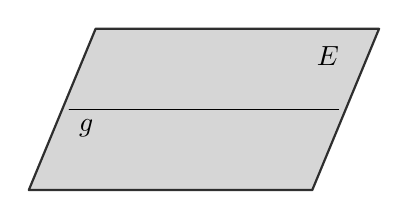
\begin{tikzpicture}[x={(-0.7071cm,-0.7071cm)}, y={(1cm,0.0cm)}, z={(0cm,1cm)}, line cap=round, line join=round,scale = 0.6]
	%Coordinates
	%Plane Vertex Points
	\coordinate (x1) at (1,-3,-1);
	\coordinate (x2) at (1,3,-1);
	\coordinate (x3) at (-1,-3,1);
        \coordinate (x4) at (-1,3,1);

        \coordinate (x5) at (0,-2.85,0);
        \coordinate (x6) at (0,2.85,0);

	
	\coordinate (O) at (0,0,0);
 
	%Plane
	\path[draw=black, fill=black!20, thick, opacity = 0.8] (x1) -- (x2) -- (x4) -- (x3) -- (x1);
	\node[shift={(-2.4,-1.5)}] at (x2) {$E$};

        \draw (x5)  node[below right] {$g$} -- (x6);

    \end{tikzpicture} \end{center} & \vspace*{25px} \begin{center} 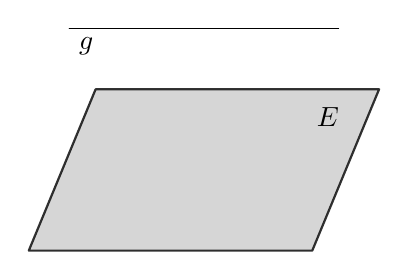
\begin{tikzpicture}[x={(-0.7071cm,-0.7071cm)}, y={(1cm,0.0cm)}, z={(0cm,1cm)}, line cap=round, line join=round,scale = 0.6]
	%Coordinates
	%Plane Vertex Points
	\coordinate (x1) at (1,-3,-1);
	\coordinate (x2) at (1,3,-1);
	\coordinate (x3) at (-1,-3,1);
        \coordinate (x4) at (-1,3,1);

        \coordinate (x5) at (0,-2.85,3);
        \coordinate (x6) at (0,2.85,3);

	
	\coordinate (O) at (0,0,0);
 
	%Plane
	\path[draw=black, fill=black!20, thick, opacity = 0.8] (x1) -- (x2) -- (x4) -- (x3) -- (x1);
	\node[shift={(-2.4,-1.5)}] at (x2) {$E$};

        \draw (x5)  node[below right] {$g$} -- (x6);

    \end{tikzpicture} \end{center}\\
    \hline
    Das LGS \newline $\vv{p} + r\vv{u} = \vv{q} + s\vv{v} + t\vv{w}$ \newline hat eine Lösung & Das LGS \newline $\vv{p} + r\vv{u} = \vv{q} + s\vv{v} + t\vv{w}$ \newline hat unendlich viele Lösungen (wahre Aussage) & Das LGS \newline $\vv{p} + r\vv{u} = \vv{q} + s\vv{v} + t\vv{w}$ \newline hat keine Lösung (falsche Aussage) \\
    \hline
    $\vv{u}$, $\vv{v}$ und $\vv{w}$ sind \newline linear unabhängig & $\vv{u}$, $\vv{v}$ und $\vv{w}$ sind \newline linear abhängig & $\vv{u}$, $\vv{v}$ und $\vv{w}$ sind \newline linear abhängig \\
    \hline
    & $\vv{q-p}$, $\vv{v}$ und $\vv{w}$ sind \newline linear abhängig & $\vv{q-p}$, $\vv{v}$ und $\vv{w}$ sind \newline linear unabhängig \\
    \hline 
    $\vv{u}$ und $\vv{n}$ sind weder orthogonal, noch parallel, d. h. \newline $\vv{u} \circ \vv{n} \neq 0$ und $\vv{u} \neq k \cdot \vv{n}$ \footnotemark & $\vv{u}$ und $\vv{n}$ sind orthogonal zueinander. d. h. \newline $\vv{u} \circ \vv{n} = 0$ & $\vv{u}$ und $\vv{n}$ sind orthogonal zueinander. d. h. \newline $\vv{u} \circ \vv{n} = 0$ \\ 
    \hline
    \end{tabular}
\end{center}

\footnotetext{Achtung Sonderfall: orthogonaler Schnitt $\rightarrow \vv{u}$ und $\vv{n}$ sind Vielfache, d. h.: $\vv{u} = k \cdot \vv{n}$}

\ \\
\ \\

Gegeben sind die Gerade $g$ mit $g: \ \vv{x} = \vv{p} + r\vv{u}$ und die Ebene $E$ in Koordinatenform mit $E: \ ax_1 + bx_2 +cx_3 = d$ 

Es gibt wieder drei Fälle, wie eine Gerade zu einer Ebene liegen kann:

\begin{tabular}{ | p{0.33\textwidth} | p{0.33\textwidth} | p{0.33\textwidth} | }
    \hline
    \begin{center} $g \cap E = \{D\}$ \end{center} & \begin{center} $g \subset E, (g \parallel E)$ \end{center}& \begin{center} $g \parallel E \land g \not\subset E$, d. h. $g \cap E = \{\}$  \end{center}\\
    \hline
    \multicolumn{3}{| p{1\textwidth} |}{\begin{center} Setze Koordinaten von $g$ in Koordinatengleichung von $E$ ein. $a\left(p_1+ru_1\right)+b\left(p_2+ru_2\right)+c\left(p_3+ru_3\right)=d$ \end{center}} \\
    \hline
    Die Gleichung \newline hat genau eine Lösung für $r$ & Die Gleichung \newline ist allgemein gültig \newline $\Rightarrow$ wahre Aussage & Die Gleichung \newline hat keine Lösung \newline $\Rightarrow$ falsche Aussage \\
    \hline
\end{tabular}

\textit{Beispiel: Bestimmung eines Schnittpunktes bei gegebener Koordinatenform}


\begin{align*}
    E_a: & \ 2ax_1 + x_2 + ax_3 = 1 \qquad ,a\in\mathbb{R} \ \footnotemark && \\
    g: & \ \vv{x} = \left(\begin{array}{c}  1 \\ 1 \\ 3 \end{array}\right) + \lambda \left(\begin{array}{c}  0 \\ -1 \\ 1 \end{array}\right) && \\
    \ \newline \\
    g \cap E_a: & \ 2a(1 + \lambda \cdot 0) + (1 + \lambda \cdot (-1)) + a(3 + \lambda \cdot 1) = 1 && \\
    & \ 2a + 1 - \lambda + 3a + a\lambda = 1 && \\
    & \ \lambda = \frac{5a}{1-a}
\end{align*}

\footnotetext{Bei $E_a$ handelt es sich um seine sog. Ebenenschar}

Für $a \neq 1$ gibt es genau einen Schnittpunkt $S$ \\
$S\left(1 \ | \ 1 - \frac{5a}{1-a} \ | \ 3 + \frac{5a}{1-a}\right)$

\ \\
\ \\
\ \\
\ \\
\ \\ 
\ \\

\section{Gegenseitige Lage von Ebenen}

Gegeben sind zwei Ebenen $E$ und $E^*$ in Koordinatenform bzw. in Normalenform. \\
Koordinatenform: $E: \  ax_1 + bx_2 + cx_3 = d$ und $E^*: \  a^*x_1 + b^*x_2 + c^*x_3 = d^*$ \\
Normalenform: $E: \ (\vv{x} - \vv{p}) \circ \vv{n} = 0$ und $E^*: \ (\vv{x} - \vv{p}) \circ \vv{n^*} = 0$ 

\begin{tabular}{ | p{0.33\textwidth} | p{0.33\textwidth} | p{0.33\textwidth} | }
    \hline
    \begin{center} $E$ und $E^*$ schneiden sich in einer Geraden \qquad $E \cap E^* = g$ \end{center} & \begin{center} $E$ und $E^*$ sind paralell zueinander $E \parallel E^* \land E \cap E^* = \{\}$ \end{center}& \begin{center} $E$ und $E^*$ sind identisch \newline \ \newline $E = E^*$  \end{center}\\
    \hline
    \begin{center} 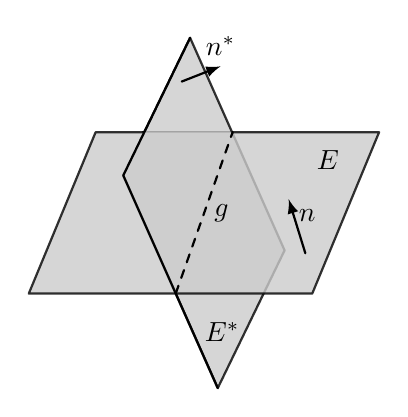
\begin{tikzpicture}[x={(-0.7071cm,-0.7071cm)}, y={(1cm,0.0cm)}, z={(0cm,1cm)}, line cap=round, line join=round,scale = 0.6]
	\coordinate (x1) at (1,-3,-1);
	\coordinate (x2) at (1,3,-1);
	\coordinate (x3) at (-1,-3,1);
        \coordinate (x4) at (-1,3,1);

        \coordinate (x4a) at (-1,-0.1,1);
        \coordinate (x4b) at (-1,-2,1);

        \coordinate (x5) at (1,1,-3);
	\coordinate (x6) at (1,-1,1.5);
	\coordinate (x8) at (-1,-1,3);
        \coordinate (x7) at (-1,1,-1.5);

        \coordinate (x8a) at (1,0.11,-1);

        \coordinate (n1a) at (1,2.5,1);
        \coordinate (n1b) at (0.5,2.5,-0.5);

        \coordinate (n2a) at (-0.75,-1,2.25);
        \coordinate (n2b) at (-0.5,0,2.75);
	
	\coordinate (O) at (0,0,0);
 
        %drawing
        
        \draw[thick] (x4a) -- (x4b);
        
        \path[draw=black, fill=black!20, thick, opacity = 0.8] (x5) -- (x6) -- (x8) -- (x7) -- (x5);
	\node[shift={(-1,-0.65)}] at (x5) {$E^*$};
 
	\path[draw=black, fill=black!20, thick, opacity = 0.8] (x4b) -- (x3) -- (x1) -- (x2)  -- (x4) -- (x4a);
	\node[shift={(-2.4,-1.5)}] at (x2) {$E$};

        \draw[thick, dashed] (x8a) -- (x4a) node[pos=0.5, right] {$g$};

        \draw[thick] (x5) -- (x6);
        \draw[thick] (x6) -- (x8);

        \draw[-latex, thick,draw=black] (n1b) -- (n1a) node[below right] {$\vv{n}$};
        \draw[-latex, thick,draw=black] (n2a) -- (n2b) node[above] {$\vv{n^*}$};
    \end{tikzpicture} \end{center} & \vspace*{25px} \begin{center} 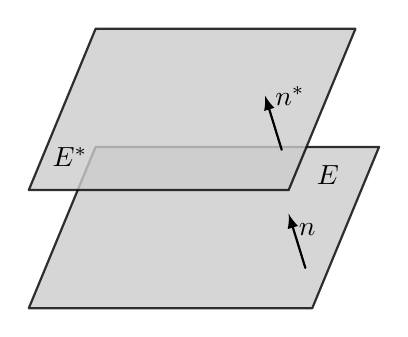
\begin{tikzpicture}[x={(-0.7071cm,-0.7071cm)}, y={(1cm,0.0cm)}, z={(0cm,1cm)}, line cap=round, line join=round,scale = 0.6]
	\coordinate (x1) at (1,-3,-1);
	\coordinate (x2) at (1,3,-1);
	\coordinate (x3) at (-1,-3,1);
        \coordinate (x4) at (-1,3,1);

        \coordinate (x5) at (1,-3,1.5);
	\coordinate (x6) at (1,2.5,1.5);
	\coordinate (x7) at (-1,-3,3.5);
        \coordinate (x8) at (-1,2.5,3.5);
        
        \coordinate (n1a) at (1,2.5,1);
        \coordinate (n1b) at (0.5,2.5,-0.5);

        \coordinate (n2a) at (1,2,3.5);
        \coordinate (n2b) at (0.5,2,2);

	
	\coordinate (O) at (0,0,0);
 
        %drawing
        \path[draw=black, fill=black!20, thick, opacity = 0.8] (x3) -- (x1) -- (x2)  -- (x4) -- (x3);
	\node[shift={(-2.4,-1.5)}] at (x2) {$E$};
 
        \path[draw=black, fill=black!20, thick, opacity = 0.8] (x5) -- (x6) -- (x8) -- (x7) -- (x5);
	\node[shift={(-0.6,0.1)}] at (x5) {$E^*$};

        \draw[-latex, thick,draw=black] (n1b) -- (n1a) node[below right] {$\vv{n}$};
        \draw[-latex, thick,draw=black] (n2b) -- (n2a) node[right] {$\vv{n^*}$};
    \end{tikzpicture} \end{center} & \vspace*{45px} \begin{center} 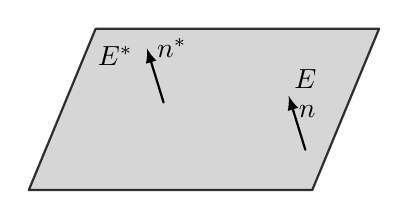
\begin{tikzpicture}[x={(-0.7071cm,-0.7071cm)}, y={(1cm,0.0cm)}, z={(0cm,1cm)}, line cap=round, line join=round,scale = 0.6]
	\coordinate (x1) at (1,-3,-1);
	\coordinate (x2) at (1,3,-1);
	\coordinate (x3) at (-1,-3,1);
        \coordinate (x4) at (-1,3,1);
        
        \coordinate (n1a) at (1,2.5,1);
        \coordinate (n1b) at (0.5,2.5,-0.5);

        \coordinate (n2a) at (1,-0.5,2);
        \coordinate (n2b) at (0.5,-0.5,0.5);

	\coordinate (O) at (0,0,0);
 
        %drawing
        \path[draw=black, fill=black!20, thick, opacity = 0.8] (x3) -- (x1) -- (x2)  -- (x4) -- (x3);
	\node[shift={(-2,-1.5)}] at (x2) {$E$} node[shift={(-2.4,-0.6)}] at (x1) {$E^*$};
 
        \draw[-latex, thick,draw=black] (n1b) -- (n1a) node[below right] {$\vv{n}$};
        \draw[-latex, thick,draw=black] (n2b) -- (n2a) node[right] {$\vv{n^*}$};
    \end{tikzpicture} \end{center} \\
    \hline
    \multicolumn{3}{| p{1\textwidth} |}{\begin{center} \textbf{1. mögliche Vorgehensweise} \end{center}} \\
    \hline
    Schreibe die zwei Gleichungen als LGS auf. \newline $ax_1 + bx_2 + cx_3 = d$ \newline $a^*x_1 + b^*x_2 + c^*x_3 = d^*$ \newline Die Lösungen für $x_1$, $x_2$ und $x_3$ beschreiben die \underline{Schnittgerade}.& Schreibe die zwei Gleichungen als LGS auf. \newline $ax_1 + bx_2 + cx_3 = d$ \newline $a^*x_1 + b^*x_2 + c^*x_3 = d^*$ \newline Das LGS hat keine Lösung (falsche Aussage).& Schreibe die zwei Gleichungen als LGS auf. \newline $ax_1 + bx_2 + cx_3 = d$ \newline $a^*x_1 + b^*x_2 + c^*x_3 = d^*$ \newline Das LGS hat unendlich viele Lösungen (wahre Aussage).\\
    \hline
    \multicolumn{3}{| p{1\textwidth} |}{\begin{center} \textbf{2. mögliche Vorgehensweise} \end{center}} \\
    \hline
    Die Vektoren $\vv{n}$ und $\vv{n^*}$ sind linear unabhängig, d. h. nicht parallel& Die Vektoren $\vv{n}$ und $\vv{n^*}$ sind linear abhängig, d. h. parallel \newline Punktprobe mit $P$ in $E^*$ bzw. mit $Q$ in $E$ ergibt eine falsche Aussage ($P \not\in E^*; Q \not\in E$)
    &  Die Vektoren $\vv{n}$ und $\vv{n^*}$ sind linear abhängig, d. h. parallel \newline Punktprobe mit $P$ in $E^*$ bzw. mit $Q$ in $E$ ergibt eine wahre Aussage ($P \in E^*; Q \in E$) \\
    \hline
\end{tabular}

Gegeben sind zwei Ebenen $E$ und $E^*$ in Parameterform. \\
$E: \ \vv{x} = \vv{p} + r\cdot \vv{u} + s\cdot \vv{v} \ ;r,s \in \mathbb{R}$ und $E^*: \ \vv{x} = \vv{p^*} + t\cdot \vv{u^*} + z\cdot \vv{v^*} \ ;t,z \in \mathbb{R}$

\begin{tabular}{ | p{0.33\textwidth} | p{0.33\textwidth} | p{0.33\textwidth} | }
    \hline
    \begin{center} $E$ und $E^*$ schneiden sich \end{center} & \begin{center} $E$ und $E^*$ sind zueinander parallel und haben keine gemeinsamen Punkte \end{center} & \begin{center} $E$ und $E^*$ sind identisch\end{center}\\
    \hline
    \begin{center} 
    \def\t{-0.9}
    \def\s{0.9}
    \def\tt{0.5}
    \def\kk{0.5}
    \def\ttt{-0.76}
    \def\sss{0.1}
    \def\tttt{-0.1}
    \def\ssss{0.1}
    \def\ttttt{-0.24}
    \def\sssss{0.9}
    \begin{tikzpicture}[x={(-0.7071cm,-0.7071cm)}, y={(1cm,0.0cm)}, z={(0cm,1cm)}, line cap=round, line join=round,scale = 0.6]
	\coordinate (x1) at (1,-3,-1);
	\coordinate (x2) at (1,3,-1);
	\coordinate (x3) at (-1,-3,1);
        \coordinate (x4) at (-1,3,1);
        \coordinate (x4a) at (-1,-0.1,1);
        \coordinate (x4b) at (-1,-2,1);
        \coordinate (x5) at (1,1,-3);
	\coordinate (x6) at (1,-1,1.5);
	\coordinate (x8) at (-1,-1,3);
        \coordinate (x7) at (-1,1,-1.5);
        \coordinate (x8a) at (1,0.11,-1);

        %Vectors Parallel to Plane
	\coordinate (n1) at ($(x4) - (x2)$);
	\coordinate (n2) at ($(x4) - (x3)$); 
        \coordinate (n3) at ($(x7) - (x5)$);
	\coordinate (n4) at ($(x7) - (x8)$); 
 
	%Points on Plane
	\coordinate (x9) at ($(x1) + \s*(n1) - \t*(n2)$);
	\node[outer sep = -0.5pt, inner sep = -0.5pt] (x10) at ($(x2) + \kk*(n1) - \tt*(n2)$) {};
	\coordinate (x11) at ($(x1) + \sss*(n1) - \ttt*(n2)$);
        \coordinate (x12) at ($(x6) + \ssss*(n3) - \tttt*(n4)$);
	\node[outer sep = -0.5pt, inner sep = -0.5pt] (x13) at ($(x5) + \kk*(n3) - \tt*(n4)$) {};
	\coordinate (x14) at ($(x6) + \sssss*(n3) - \ttttt*(n4)$);
	\coordinate (O) at (0,0,0);
 
        %drawing
        \draw[thick] (x4a) -- (x4b);
        \path[draw=black, fill=black!20, thick, opacity = 0.8] (x5) -- (x6) -- (x8) -- (x7) -- (x5);
	\node[shift={(-1,-0.65)}] at (x5) {$E^*$};
	\path[draw=black, fill=black!20, thick, opacity = 0.8] (x4b) -- (x3) -- (x1) -- (x2)  -- (x4) -- (x4a);
	\node[above right] at (x1) {$E$};
        \draw[thick] (x8a) -- (x4a);
        \draw[thick] (x5) -- (x6);
        \draw[thick] (x6) -- (x8);
        \draw[-latex, thick,draw=blue] (x10) -- (x9) node[blue, pos=0.6, above] {$\vb{\vv{v}}$};
        \draw[-latex, thick,draw=red] (x10) -- (x11) node[red, pos=0.6, above] {$\vb{\vv{u}}$};
        \draw[-latex, thick,draw=red] (x13) -- (x12) node[red, pos=0.6, below] {$\vb{\vv{u^*}}$};
        \draw[-latex, thick,draw=blue] (x13) -- (x14) node[blue, pos=0.6, left] {$\vb{\vv{v^*}}$};
    \end{tikzpicture} \end{center} & 
    \begin{center} \def\t{0.8}
    \def\s{0.2}
    \def\ss{0.6}
    \def\sss{0.8}
    \def\ttt{0.6}
    \def\ssss{0.1}
    \def\tttt{0.5}
    \def\ttttt{0.4}
    \begin{tikzpicture}[x={(-0.7071cm,-0.7071cm)}, y={(1cm,0.0cm)}, z={(0cm,1cm)}, line cap=round, line join=round,scale = 0.6]
	\coordinate (x1) at (1,1,1);
	\coordinate (x2) at (1,5,2);
        \coordinate (x3) at (-1,5,2);
	\coordinate (x4) at (-1,1,1);
        \coordinate (x5) at (1,1,3);
	\coordinate (x6) at (1,5,4);
        \coordinate (x7) at (-1,5,4);
	\coordinate (x8) at (-1,1,3);
        \coordinate (O) at (0,3,-3);

        %Vectors Parallel to Plane
	\coordinate (n1) at ($(x3) - (x2)$);
	\coordinate (n2) at ($(x3) - (x4)$); 
        \coordinate (n3) at ($(x7) - (x6)$);
	\coordinate (n4) at ($(x7) - (x8)$); 
 
	%Points on Plane
	\node[outer sep = -0.5pt, inner sep = -0.5pt] (x9) at ($(x2) + \s*(n1) - \t*(n2)$) {};
	\node[outer sep = -0.5pt, inner sep = -0.5pt] (x10) at ($(x6) + \ss*(n3) - \t*(n4)$) {};
        \coordinate (x11) at ($(x2) + \sss*(n1) - \ttt*(n2)$);
        \coordinate (x12) at ($(x2) + \ssss*(n1) - \tttt*(n2)$);
        \coordinate (x13) at ($(x6) + \sss*(n3) - \ttttt*(n4)$);
        \coordinate (x14) at ($(x6) + \ssss*(n3) - \ttttt*(n4)$);
 
        %drawing
        \draw[-latex, thick,draw=magenta] (O) node[right] {$O$} -- (x9) node[magenta, pos=0.2, left] {$\vv{p}$};
        \draw[-latex, thick,draw=magenta] (O) -- (x10) node[magenta, pos=0.2, right] {$\vv{p^*}$}; 
        \path[draw=black, fill=black!20, thick, opacity = 0.8] (x1) -- (x2) -- (x3) -- (x4) -- (x1);
	\node[right] at (x3) {$E$};
        \draw[-latex, thick,draw=magenta] (x9) -- (x10) node[magenta, pos = 0.5, left] {$\vv{p^*} - \vv{p}$};
        \path[draw=black, fill=black!20, thick, opacity = 0.8] (x5) -- (x6) -- (x7) -- (x8) -- (x5);
	\node[right] at (x7) {$E^*$};
        \draw (x10) circle (1pt) node[magenta, left] {$P^*$};
        \draw (x9) circle (1pt) node[magenta, left] {$P$};
        \draw[-latex, thick,draw=red] (x9) -- (x11) node[red, right] {$\vv{u}$};
        \draw[-latex, thick,draw=blue] (x9) -- (x12) node[blue, shift={(-0.25,0)}] {$\vv{v}$};
        \draw[-latex, thick,draw=red] (x10) -- (x13) node[red, right] {$\vv{u^*}$};
        \draw[-latex, thick,draw=blue] (x10) -- (x14) node[blue, shift={(-0.25,0)}] {$\vv{v^*}$};
        \draw (O) circle (1pt);
    \end{tikzpicture} \end{center} & \begin{center} \def\t{0.8}
    \def\s{0.2}
    \def\ss{0.8}
    \def\sss{0.5}
    \def\ttt{0.6}
    \def\ssss{0.1}
    \def\tttt{0.5}
    \def\sssss{0.5}
    \def\ttttt{0.15}
    \def\ssssss{0.95}
    \def\tttttt{0.4}
    \begin{tikzpicture}[x={(-0.7071cm,-0.7071cm)}, y={(1cm,0.0cm)}, z={(0cm,1cm)}, line cap=round, line join=round,scale = 0.6]
        \coordinate (x1) at (1.5,1,1);
        \coordinate (x2) at (1.5,6,2);
        \coordinate (x3) at (-2,6,2);
        \coordinate (x4) at (-2,1,1);
        \coordinate (O) at (0,3,-3);
    
        %Vectors Parallel to Plane
        \coordinate (n1) at ($(x3) - (x2)$);
        \coordinate (n2) at ($(x3) - (x4)$); 
     
        %Points on Plane
        \node[outer sep = -0.5pt, inner sep = -0.5pt] (x9) at ($(x2) + \s*(n1) - \t*(n2)$) {};
        \node[outer sep = -0.5pt, inner sep = -0.5pt] (x10) at ($(x2) + \ss*(n1) - \tt*(n2)$) {};
        \coordinate (x11) at ($(x2) + \sss*(n1) - \ttt*(n2)$);
        \coordinate (x12) at ($(x2) + \ssss*(n1) - \tttt*(n2)$);
        \coordinate (x13) at ($(x2) + \sssss*(n1) - \ttttt*(n2)$);
        \coordinate (x14) at ($(x2) + \ssssss*(n1) - \tttttt*(n2)$);
    	
        %drawing
        \draw[-latex, thick,draw=magenta] (O) node[right] {$O$} -- (x9) node[magenta, pos=0.2, left] {$\vv{p}$};
        \draw[-latex, thick,draw=magenta] (O) node[right] {$O$} -- (x10) node[magenta, pos=0.2, right] {$\vv{p^*}$};
        \path[draw=black, fill=black!20, thick, opacity = 0.8] (x1) -- (x2) -- (x3) -- (x4) -- (x1);
        \node[shift={(0.45,-0.3)}] at (x3) {$E$};
        \node[above] at (x2) {$E^*$};
        \draw (x9) circle (1pt) node[magenta, left] {$P$};
        \draw (x10) circle (1pt) node[magenta, left] {$P^*$};
        \draw[-latex, thick,draw=red] (x9) -- (x11) node[red, right] {$\vv{u}$};
        \draw[-latex, thick,draw=blue] (x9) -- (x12) node[blue, shift={(-0.25,0)}] {$\vv{v}$};
        \draw[-latex, thick,draw=red] (x10) -- (x14) node[red, above] {$\vv{u^*}$};
        \draw[-latex, thick,draw=blue] (x10) -- (x13) node[blue, shift={(-0.25,0)}] {$\vv{v^*}$};
        \draw[-latex, thick, magenta] (x9) -- (x10) node[magenta, pos = 0.6, left] {$\vv{p^*} - \vv{p}$};
        \draw (O) circle (1pt);
    \end{tikzpicture}\end{center}\\
    \hline
    $\vv{u}$, $\vv{v}$, $\vv{u^*}$  \textbf{oder} $\vv{u}$, $\vv{v}$, $\vv{v^*}$ \newline sind linear unabhängig & \multicolumn{2}{c|}{$\vv{u}$, $\vv{v}$, $\vv{u^*}$  \textbf{und} $\vv{u}$, $\vv{v}$, $\vv{v^*}$ sind linear abhängig}\\
    \hline
    & $\vv{p} - \vv{p^*}$, ?, $\vv{v}$ \newline sind linear unabhängig & $\vv{p} - \vv{p^*}$, ?, $\vv{v}$ \newline sind linear abhängig \\
    \hline
    \multicolumn{3}{| p{1\textwidth} |}{\begin{center} \textbf{3. mögliche Vorgehensweise} \end{center}} \\
    \hline
    Die Gleichung \newline $\vv{p} + r \vv{u} + s \vv{v} = \vv{p^*} + t \vv{u^*} + z \vv{v^*}$ \newline hat unendlich viele Lösungen (ist noch abhängig von einem Parameter). & Die Gleichung \newline $\vv{p} + r \vv{u} + s \vv{v} = \vv{p^*} + t \vv{u^*} + z \vv{v^*}$ \newline hat keine Lösung. LGS ergiebt eine flasche Aussage. &  Die Gleichung \newline $\vv{p} + r \vv{u} + s \vv{v} = \vv{p^*} + t \vv{u^*} + z \vv{v^*}$ hat unendlich viele Lösungen. LGS ergibt eine wahre Aussage. \\
    \hline
\end{tabular}

Um die Lagebeziehung zweier Ebenen zu untersuchen, sind die Normalengleichung oder die Koordinatengleichung am geschicktesten.

Hat man hingegen die Parametergleichung gegeben, so wandeln wir diese zuerst in eine der beiden anderen Darstellungsformen um. Zuerst untersuchen wir, ob die Normalenvektoren Vielfache sind und führen dann gegebenenfalls noch eine Punktprobe durch, um zu entscheiden, ob die Ebenen außer zueinander parallel zudem identisch sind.

Um die Schnittgerade zweier Ebenen zu bestimmen, muss ein LGS gelöst werden.

\textit{Beispiel:} Gegeben ist die Schar der Ebenen $E_a: \ 2ax_1 + x_2 + ax_3 = 1 \ , a \in \mathbb{R}$. Zeigen Sie, dass es eine Gerade $h$ gibt, die in allen Ebenen der Schar liegt.

\begin{align}
    E_0 \cap E_1 = \{h\} \tag{1} 
\end{align}
\begin{align*}
    &E_0: \ x_2 && = 1 & \\
    &E_1: \ 2x_1  +  x_2  +   x_3  && = 1 & \\
    \ \\
    & E_0 \cap E_1 : x_2 && = 1 \\   
    &2x_1 + 1  +x_3 && = 1  \\
    &2x_1 +x_3 && = 0 
\end{align*}

Setze: $x_1 = t \ ,t \in \mathbb{R}$

Damit: $x_2 = 1$ und $x_3 = -2t$

$g: \ \vv{x} = \left(\begin{array}{c}  0 \\1 \\ 0 \end{array}\right) + t \left(\begin{array}{c}  1 \\ 0 \\ -2 \end{array}\right) \, t \in \mathbb{R}$

\begin{align}
    g \text{ in } E_a \tag{2}
\end{align}
\begin{align*}
    & 2a\cdot t + 1 + a\cdot (-2t) && = 1 &\\
    & 2at + 1 -2at && = 1 &\\
    & 1 && = 1 &
\end{align*}

$\Rightarrow$ wahre Aussage $\Rightarrow$ $g$ liegt in allen Ebenen der Schar